\documentclass[conference]{IEEEtran}
\IEEEoverridecommandlockouts
% The preceding line is only needed to identify funding in the first footnote. If that is unneeded, please comment it out.
%Template version as of 6/27/2024
\usepackage{algorithm}
\usepackage{booktabs}
\usepackage{float}
\usepackage{algpseudocode}
\usepackage{cite}
\usepackage{amsmath,amssymb,amsfonts}
% \usepackage{algorithmic}
\usepackage{graphicx}
\usepackage{textcomp}
\usepackage{xcolor}
\def\BibTeX{{\rm B\kern-.05em{\sc i\kern-.025em b}\kern-.08em
    T\kern-.1667em\lower.7ex\hbox{E}\kern-.125emX}}
\begin{document}

\title{Hidden Markov models in the sequential detection of auditory steady-state responses: A comparison with the Rayleigh test}

\author{\IEEEauthorblockN{1\textsuperscript{st} Victor Hugo de Souza Singulani Ragazzi}
\IEEEauthorblockA{\textit{Department of Electrical Engineering} \\
\textit{Federal University of Viçosa}\\
Viçosa, Brazil \\
victor.ragazzi@ufv.br}
}

\maketitle

\begin{abstract}
Sequential testing strategies are commonly used to reduce the time of automated detection of an auditory steady-state response (ASSR). In these strategies, each application of the test is compared with a critical value, without considering how the statistic evolved along the exam. The objective of this work is to evaluate whether a Hidden Markov Model (HMM) with two hidden states, response absent and response present, improves the detection when the Rayleigh test statistic is used as its observation. Instead of a discrete observation matrix, each state is described by a Gamma probability density function, and the density of the present state is obtained from a hierarchical Bayesian model sampled by Markov chain Monte Carlo. The method was evaluated on recordings of eleven normal-hearing adults, leaving one participant out at a time. With each recording analyzed separately, the HMM reached a detection rate of 54.1\% against 55.9\% of the Rayleigh test, with similar false positive rate (8.3\% and 8.5\%) and detection time, and no difference was significant. When the recordings of a participant were analyzed as one sequence, the HMM detected 58.2\% against 51.6\%, with a higher false positive rate (8.9\% against 6.1\%). The HMM adds little when the observation already accumulates the evidence of the exam, and becomes useful when information can be carried from one recording to the next.
\end{abstract}

\begin{IEEEkeywords}
Electroencephalogram, auditory steady-state response, sequential tests, hidden Markov model, Bayesian inference, false positive.
\end{IEEEkeywords}

\section{Introduction}

Auditory evaluation is a crucial step in the diagnosis and treatment of hearing problems, especially in children. According to the Joint Committee on Infant Hearing \cite{jcih2007}, the electrophysiological auditory evaluation is recommended by the third month of life, aiming to start the treatment as soon as possible in case of risk of hearing loss. The need to expedite auditory evaluation is evident to optimize the time of professionals and patients, minimizing costs and preventing hearing difficulties.

For small children, babies and uncooperative individuals, it is recommended to use objective audiometry, such as Otoacoustic Emissions (OAE) or the Auditory Brainstem Response (ABR) \cite{picton2003}. Within these techniques, the Auditory Steady-State Response (ASSR) evaluation emerges as a complement to the ABR and OAE strategies \cite{sturzebecher1999}. ASSR can estimate hearing at different frequencies simultaneously, which makes it particularly useful for identifying hearing losses in specific frequencies \cite{sininger2018}. The response is an evoked potential detected in the electroencephalogram (EEG).

The detection of ASSRs in EEG signals is conducted by statistical procedures in the time or frequency domain, known as Objective Response Detectors (ORD) \cite{sturzebecher1999}. The test can be applied once at the end of the EEG collection (Single-Shot) or performed before the complete collection of the signal and repeated at defined time intervals. In this strategy of sequential tests, the process repeats until it identifies a response or reaches the time limit, which allows for a reduction in detection time \cite{zanotelli2020,vaz2024,cebulla2015,chesnaye2020}.

One characteristic of sequential tests is the increase in the false positive rate (FP) as the number of detection attempts increases. To control the FP rate, the critical value of the test is raised, either by the Bonferroni correction, which is conservative because the repeated tests are not independent, or by Monte Carlo simulations \cite{sturzebecher2005}.

In all these strategies, each application of the test is judged against a critical value. The decision does not take into account how the statistic evolved along the exam, and only the behavior of the test in the absence of response is modeled. A Hidden Markov Model (HMM) offers a different view of the same problem: a state that cannot be observed directly, here the absence or presence of a response, generates a sequence of observations, and the state is inferred from the whole sequence \cite{rabiner1989}.

This study's primary objective is to evaluate whether using the Rayleigh test statistic as the observation of a two-state HMM improves the detection rate, or shortens the detection time, in relation to the test applied alone, without increasing the FP rate. The observation matrix of the HMM is replaced by probability density functions, one for each state, and the density of the state with response is estimated with a hierarchical Bayesian model.

\section{Background}

\subsection{Detection of the ASSR}

An ASSR evoked by a tone modulated at frequency $f_m$ appears in the EEG spectrum as a component at $f_m$ whose phase repeats from one epoch to the next. ORDs in the frequency domain test this regularity using the phase, the amplitude or both \cite{dobie1993,sturzebecher1999,cebulla2006}. The Rayleigh test uses only the phase: without a response the phases are uniformly distributed, and with a response they concentrate around a preferred direction \cite{mardia2000}.

For sequential application, Stürzebecher et al. \cite{sturzebecher2005} obtained by simulation a constant critical value that keeps the FP rate at the nominal level. Later strategies added higher harmonics to the detector \cite{cebulla2006}, a critical value that grows at each test stage \cite{sturzebecher2013} and a variable interval between tests \cite{cebulla2015}. Other authors proposed stopping rules based on the number of consecutive detections \cite{zanotelli2020}, group sequential tests \cite{chesnaye2020} and criteria to stop the exam when no response is expected \cite{vaz2024}. All of them compare a statistic with a critical value calibrated under the hypothesis of no response.

\subsection{Hidden Markov models}

An HMM is defined by the initial state probabilities $\pi$, the state transition matrix $A$ and the observation distribution $B$ of each state \cite{rabiner1989}. When the observations are continuous, $B$ is a set of probability density functions instead of a matrix. Given a sequence of observations, the Viterbi algorithm finds the most probable sequence of hidden states \cite{viterbi1967}. HMMs have been applied to EEG in problems in which a state lasts for some time, such as the online classification of single trials in brain-computer interfaces \cite{obermaier2001}.

In the detection of the ASSR, the closest approach found is the use of a Kalman filter, another state-space model, to estimate the amplitude and phase of the response along the exam \cite{luke2017}. In the literature search conducted for this work, no study was found that applies an HMM to the detection of the ASSR.

\section{Methodology}

\subsection{Observation: cumulative Rayleigh statistic}

The EEG is divided into epochs of one second and the Fourier transform of each epoch gives the phase $\theta_i$ at the modulation frequency. With $N$ epochs collected, the Rayleigh statistic is
\begin{equation}
Z_N=\frac{1}{N}\left|\sum_{i=1}^{N}e^{j\theta_i}\right|^2 .
\label{eq:z}
\end{equation}
Without a response, $Z_N$ follows approximately an exponential distribution with mean one for any $N$, and the p-value of the test is $p=e^{-Z_N}$ \cite{mardia2000}. With a response, the phases have a preferred direction and the expected value of the statistic grows with the number of epochs:
\begin{equation}
E[Z_N]=1+(N-1)\rho ,
\label{eq:media}
\end{equation}
in which $\rho$, between 0 and 1, is the squared length of the mean phase vector and measures the strength of the response.

The statistic is recomputed at every $M_{step}=10$ new epochs, always with all the epochs collected since the beginning. The sequence $Z_{10}, Z_{20}, Z_{30},\ldots$ is the observation of both the Rayleigh test and the HMM.

\subsection{HMM with density functions as observation model}

The HMM has two hidden states, response Absent ($\mathcal{A}$) and response Present ($\mathcal{P}$), an initial probability $\pi$ of the Present state and a $2\times2$ transition matrix $A$. Each state has a Gamma density, written here with shape $k$ and mean $\mu$:
\begin{align}
b_{\mathcal{A}}(z) &= \mathrm{Gamma}(z \mid k_0,\ \mu_0), \label{eq:aus}\\
b_{\mathcal{P}}(z \mid N) &= \mathrm{Gamma}\big(z \mid k,\ 1+(N-1)\rho\big). \label{eq:pres}
\end{align}
The Gamma family contains the exponential distribution expected without a response ($k_0=\mu_0=1$). The Absent density is fixed, while the Present density moves to the right as the exam proceeds, following \eqref{eq:media}. The same value of $Z$ can therefore support different states at different moments of the exam.

\begin{figure*}[t]
\centering
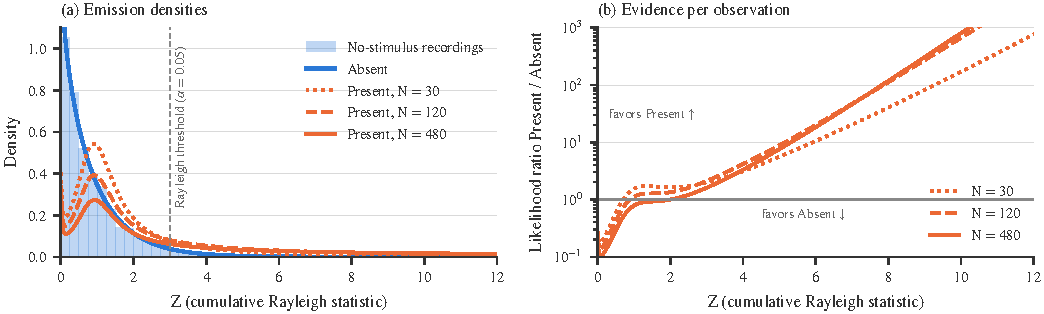
\includegraphics[width=0.8\textwidth]{figuras/fig_emissoes.pdf}
\caption{Observation model of the HMM, fitted with all participants. (a) Density of each state; the histogram shows the values of $Z$ in the recordings without stimulation, and the Present density is drawn for three numbers of epochs $N$. (b) Ratio between the Present and Absent densities, in logarithmic scale.}
\label{fig:emissoes}
\end{figure*}

\subsection{Hierarchical Bayesian model of the Present state}

The response does not have the same strength in every exam. Instead of fixing $k$ and $\rho$, each calibration sequence $s$ has its own pair $(k_s,\rho_s)$, drawn from population distributions:
\begin{equation}
\begin{aligned}
Z_{s,t}\mid k_s,\rho_s &\sim \mathrm{Gamma}\big(k_s,\ 1+(N_{s,t}-1)\rho_s\big),\\
k_s \sim \mathrm{Gamma}&(a_k,b_k),\qquad \rho_s \sim \mathrm{Gamma}(a_\rho,b_\rho),
\end{aligned}
\label{eq:hier}
\end{equation}
with shape $a$ and rate $b$. The four hyperparameters receive a prior that is uniform in the logarithm, $p(a)\propto 1/a$.

The joint posterior of the hyperparameters and of all pairs $(k_s,\rho_s)$ has no closed form and was sampled by Markov chain Monte Carlo (MCMC) \cite{gelman2013}. The rates $b_k$ and $b_\rho$ have Gamma full conditionals and were drawn by Gibbs sampling; the remaining parameters were updated by random-walk Metropolis steps in the logarithmic scale. Four chains ran for 20\,000 iterations, with the first 5\,000 discarded and one in every ten of the remaining kept. Convergence was checked with the $\hat{R}$ statistic \cite{gelman1992}.

The density used by the HMM is the posterior predictive density of a new exam. For each of $M=2000$ posterior draws of the hyperparameters, one pair $(k_m,\rho_m)$ is drawn from \eqref{eq:hier}, and
\begin{equation}
b_{\mathcal{P}}(z\mid N)\approx\frac{1}{M}\sum_{m=1}^{M}\mathrm{Gamma}\big(z\mid k_m,\ 1+(N-1)\rho_m\big).
\label{eq:pred}
\end{equation}
Nothing is learned during the exam: after calibration, \eqref{eq:aus} and \eqref{eq:pred} are fixed curves.

\subsection{Decision}

At each evaluation $t$, the Viterbi algorithm is applied to the observations collected so far, $Z_{10},\ldots,Z_{10t}$, combining $\pi$, $A$ and the two densities. The evaluation is counted as positive if the most probable sequence of states contains the Present state. For the Rayleigh test, the evaluation is positive if $p\le\alpha$.

The exam stops, with a detection, at the first evaluation in which a stopping rule is satisfied. The rules considered require a minimum number of consecutive positive evaluations, a minimum fraction of positive evaluations so far, or a combination of both (144 rules). No rule can stop the exam before the third evaluation (30 s).

\section{Experiments}

\subsection{Data}

Eleven adult individuals participated in the study, consisting of two women and nine men, aged between 20 and 35 years, with hearing considered normal (threshold $\le$ 20 dB Hearing Level). The carrier frequencies for both ears were the same: 500, 1000, 2000 and 4000 Hz, modulated respectively at 81, 85, 89 and 93 Hz for the right ear and 83, 87, 91 and 95 Hz for the left ear. The research received approval from the local Ethics Committee (CEP/UFV No. 2.105.334), and all volunteers signed an informed consent form. Data collection took place in an acoustically isolated booth. The EEG was acquired with sixteen electrodes arranged according to the International System 10-20, at 1000 or 1750 Hz per channel, and divided into one-second epochs.

Each volunteer was recorded in six conditions: stimulation at 30, 40, 50, 60 and 70 dB SPL and one recording without stimulation. The recordings last approximately 8 minutes at 30 and 40 dB, 5 minutes at 50 dB, 2 to 3 minutes at 60 dB and 1 minute at 70 dB; the recordings without stimulation last from 30 s to 5 minutes. Only the FC electrode was analyzed, without artifact rejection.

Each combination of participant, condition and frequency is treated as an independent exam. There are 440 exams with a response expected (5 intensities, 8 modulation frequencies, 11 participants). The FP rate was measured in two ways: in the 8 frequencies neighboring the modulation frequencies (82, 84, \ldots, 96 Hz) of all recordings, where no response exists (528 exams), and in the modulation frequencies of the recordings without stimulation (88 exams).

\begin{figure*}[t]
\centering
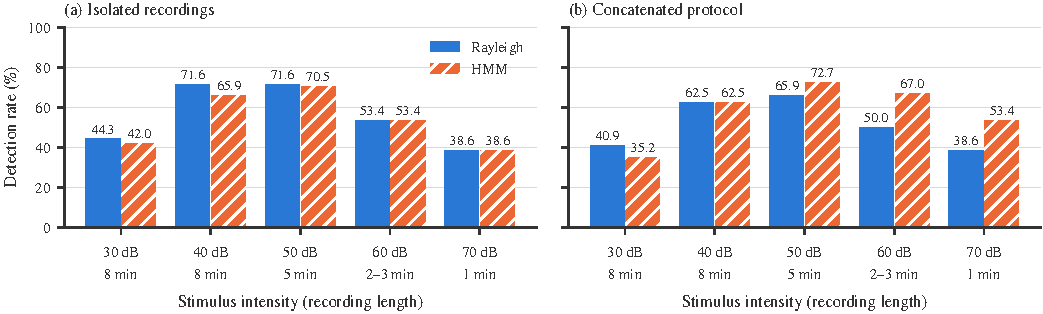
\includegraphics[width=0.8\textwidth]{figuras/fig_deteccao.pdf}
\caption{Detection rate by stimulus intensity, leaving one participant out. (a) Each recording analyzed as an independent exam. (b) Recordings of each participant analyzed as one sequence, from no stimulus to 70 dB. The recording length is shown below each intensity.}
\label{fig:deteccao}
\end{figure*}

\subsection{Calibration and validation}

The Absent density \eqref{eq:aus} was fitted by maximum likelihood to the values of $Z$ of the recordings without stimulation. The Present model \eqref{eq:hier} was calibrated with the sequences of $Z$ of all recordings with stimulation: since every participant has normal hearing, all of them were counted as response present.

The values of $\pi$, $A$ and the stopping rule were chosen by grid search (12 values of $\pi$, 12 and 9 values for the two transition probabilities, 144 rules), maximizing the detection rate subject to an FP rate in the neighboring frequencies not higher than that of the reference detector. The reference is the Rayleigh test with $\alpha=0.05$ and detection after three consecutive significant tests.

The validation left one participant out at a time. In each of the eleven rounds, the densities, $\pi$, $A$, the stopping rule and the FP limit were obtained only from the other ten participants and then applied to the participant left out.

\subsection{Experiments and performance measures}

Three experiments were carried out. (i) \textit{Isolated recordings}: the HMM is compared with the reference detector, each recording being one exam. (ii) \textit{Fixed density}: the validation is repeated replacing \eqref{eq:pred} by a single Gamma density, with one pair $(k,\rho)$ fitted by maximum likelihood to all calibration sequences, to measure what the hierarchical Bayesian model adds. (iii) \textit{Concatenated protocol}: the recordings of a participant are analyzed, for each frequency, as one sequence in the order no stimulus, 30, 40, 50, 60 and 70 dB. The statistic $Z$ restarts at each recording for both detectors, but the HMM keeps its state from one recording to the next. Each intensity is still decided separately, by the current state of the most probable path. In this exploratory experiment the hyperparameters were fixed at their maximum likelihood values, $\alpha$ and the stopping rule of the Rayleigh test were also searched, and both detectors were limited to an FP rate of 6\% in the calibration participants.

The detection rate is the proportion of exams with stimulation in which a response was detected, and the detection time is the number of epochs collected until the detection. Detection and FP rates of two detectors were compared with the exact McNemar test, and detection times with the Wilcoxon signed-rank test in the exams detected by both.

\section{Results}

\subsection{Estimated densities}

The Absent density fitted to the recordings without stimulation ($k_0=0.91$, $\mu_0=0.87$) is close to the theoretical exponential. In the Present model, the chains agreed ($\hat{R}\le1.002$ for the hyperparameters in all rounds). With all participants, the posterior means and standard deviations were $a_k=1.46\pm0.11$, $b_k=0.32\pm0.03$, $a_\rho=0.29\pm0.02$ and $b_\rho=9.5\pm1.1$. The shape of the distribution of $\rho$ below one means that the strength of the response is very unequal between exams: its mean is 0.031, but half of the exams have $\rho$ below 0.007.

Fig.~\ref{fig:emissoes} shows the resulting densities. Because many stimulated recordings have a weak response, the Present density keeps a large part of its mass in the same region as the Absent one, and differs mainly by a long tail that grows with $N$. The ratio between the two densities is the evidence that one observation brings. With $N=120$, a value $Z=6$ is 20 times more probable under Present, while $Z=1$ is almost neutral (1.1). After 480 epochs, a low value such as $Z=0.5$ becomes evidence of absence, being 3.4 times more probable under Absent.

\subsection{Isolated recordings}

Table~\ref{tab:geral} presents the performance of the detectors. The HMM detected 54.1\% of the responses and the Rayleigh test 55.9\%. In 14 exams only the Rayleigh test detected the response and in 6 only the HMM, a difference that is not significant ($p=0.12$). The FP rate in the neighboring frequencies was practically the same (8.3\% and 8.5\%, $p=1.00$). In the recordings without stimulation the HMM had 6.8\% against 3.4\%, which corresponds to three exams and is also not significant ($p=0.25$).

The median detection time was 80 s for the HMM and 95 s for the Rayleigh test. This difference comes mostly from the exams that each detector finds: in the 232 exams detected by both, the mean difference was 0.9 s ($p=0.68$).

\begin{table}[t]
\caption{Performance of the detectors, leaving one participant out}
\label{tab:geral}
\centering
\setlength{\tabcolsep}{3.5pt}
\begin{tabular}{@{}lcccc@{}}
\toprule
 & Detection & \multicolumn{2}{c}{False positives} & Time (s) \\
\cmidrule(lr){3-4}
Detector & rate & Neighbor & No stim. & mean / median \\
\midrule
\multicolumn{5}{@{}l}{\textit{Isolated recordings}}\\
Rayleigh (ref.) & 55.9\% & 8.5\% & 3.4\% & 133 / 95 \\
HMM, Bayesian & 54.1\% & 8.3\% & 6.8\% & 125 / 80 \\
HMM, fixed & 54.5\% & 8.3\% & 6.8\% & 127 / 90 \\
\midrule
\multicolumn{5}{@{}l}{\textit{Concatenated protocol}}\\
Rayleigh & 51.6\% & 6.1\% & 5.7\% & 125 / 80 \\
HMM & 58.2\% & 8.9\% & 2.3\% & 102 / 30 \\
\bottomrule
\end{tabular}
\end{table}

Fig.~\ref{fig:deteccao}(a) separates the detection rate by intensity. The two detectors follow the same profile: the rate rises from 30 to 50 dB and falls at 60 and 70 dB, whose recordings are much shorter and give a sequential test fewer opportunities to detect. The only visible difference is at 40 dB.

The search chose similar parameters in all rounds: initial probability of the Present state between 0.1 and 0.3 and, in ten of the eleven rounds, a probability of returning from Present to Absent of 0.5, the largest value of the grid.

\subsection{Fixed density}

Replacing the Bayesian density by a single Gamma ($k$ between 0.81 and 0.90 and $\rho$ between 0.010 and 0.013 across rounds) did not change the performance (Table~\ref{tab:geral}). The two versions disagreed in only 8 of the 440 exams with stimulation ($p=0.73$), had the same FP rates and no significant difference in detection time ($p=0.34$).

\subsection{Concatenated protocol}

When the recordings were analyzed as one sequence, the HMM detected 58.2\% of the responses against 51.6\% of the Rayleigh test ($p=0.001$). Fig.~\ref{fig:deteccao}(b) shows that the gain is concentrated in the short recordings: 67.0\% against 50.0\% at 60 dB and 53.4\% against 38.6\% at 70 dB. At 30 dB, the first recording with stimulation, the HMM detected less (35.2\% against 40.9\%).

The gain had a cost. The FP rate in the neighboring frequencies was higher for the HMM (8.9\% against 6.1\%, $p=0.03$), although both were calibrated under the same limit. In addition, at 70 dB, 44 of the 47 detections of the HMM occurred at the first evaluation allowed, 30 s after the beginning of the recording. These detections are inherited from the state reached at 60 dB more than they are supported by new data.

\section{Discussion and conclusions}

With each recording treated as one exam, the HMM did not improve on the Rayleigh test: detection rate, FP rate and detection time were statistically equal. The result is explained by the observation chosen. The cumulative statistic already summarizes all the epochs collected, so $Z_{20}$ contains the epochs of $Z_{10}$. The observations are far from independent given the state, as the HMM assumes, and the sequence has little to add to its last value. The parameters selected point in the same direction: with a probability of 0.5 of leaving the Present state, the model keeps almost no memory, and its decision approaches a comparison of the last $Z$ with a threshold that depends on $N$.

The estimated densities also limit the gain. Counting every stimulated recording as a response includes exams in which the response is too weak to be seen, and these pull the Present density toward the Absent one (Fig.~\ref{fig:emissoes}). The equality between the Bayesian and the fixed density indicates that the detection is limited by the information contained in $Z$, and not by the level of detail with which its distribution is described.

The concatenated protocol shows where the hidden state helps. A response found at one intensity makes a response at the next intensity more likely, and this is information that a test restarted at each recording cannot use. The HMM used it to detect earlier and more often in recordings too short for the Rayleigh test. The same memory, however, carries errors forward, which appeared as a higher FP rate.

Some limitations should be considered. The study has only eleven normal-hearing adults, so the rates are not clinical estimates. The values of $\pi$ and $A$ were selected in a grid, with one of them at its limit, and the concatenated protocol is exploratory.

In summary, the results of this study demonstrate that replacing the critical value of a sequential Rayleigh test by an HMM does not improve the detection of the ASSR when the observation is the cumulative statistic itself, with or without a Bayesian observation model. The HMM becomes advantageous when the exam is seen as a sequence of recordings, at the price of more false positives. Future work should use observations that do not share epochs, such as the phase of each window, and control the FP rate of the concatenated protocol before it is considered for objective audiometry.

\bibliographystyle{IEEEtran}
\bibliography{reference}

\end{document}
